\section{LLM-Based Authoring Assistant}

\subsection{Introduction}

\begin{itemize}
    \item \textbf{QueryContext}: Represents the input, containing dataset details (path and variable name), library imports, code, and paragraphs (lists of strings and fluid expressions).
    \item \textbf{Fluid Generator}: Receives the QueryContext and requests the LLM to generate a Fluid Expression.
    \item \textbf{Fluid Evaluator}: Verifies the Fluid Expression syntactically and semantically. It runs through the fluid compiler, comparing the output with the expected value. Errors are sent back to the LLM for regeneration if needed.
\end{itemize}

\subsection{Candidate Research Questions}

\subsubsection{Usability of LLM-based authoring tool vs.~editing purely by hand}

\subsubsection{Impact of documentation and naming conventions on the output accuracy}
Analyze how the use of proper naming conventions and the inclusion of comments in each example of the
in-context learning dataset affect the accuracy of the LLM's output. \textbf{RQ}: How do documentation, naming
conventions, affect performance of LLM?

\subsubsection{Impact of Example Complexity on LLM Generalization in DSLs}
Analyse the impact of the structure of the in-context learning dataset on the accuracy of responses, with a
particular focus on the complexity of datasets. By complexity, we mean the number of Fluid elements that the
in-context learning dataset contains for each example.

\begin{figure}
    \centering
    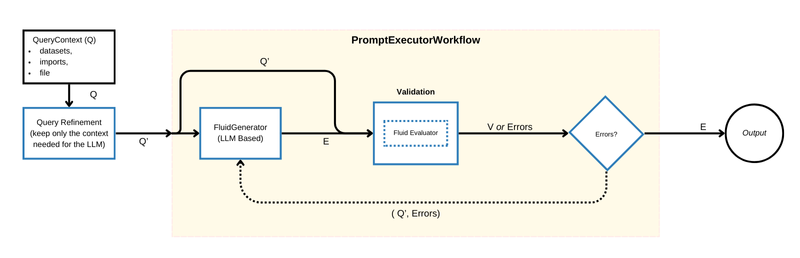
\includegraphics[width=0.95\linewidth]{fig/authoring-assistant-architecture.png}
    \caption{Draft architecture of the LLM-based code generation}
    \label{fig:authoring-assistant-architecture}
\end{figure}

\textbf{Related work (links)}
\begin{itemize}
    \item \href{http://www.lrec-conf.org/proceedings/lrec-coling-2024/pdf/2024.main-1.1251.pdf}{Scaling Data Diversity for Fine-Tuning Language Models in Human Alignment} - not strongly related to dsl, but interesting about diversity in prompt.
\end{itemize}

\textbf{RQ}: What is the impact of example complexity on the accuracy of LLM-generated outputs in DSL tasks?

\subsubsection{Analysis of the Role of Formal Models in Enhancing LLMs for DSL Generation}

Analyse the impact of formal models, such as Context-Free Grammar, on the responses generated by the LLM.

\textbf{Related work (links)}
\begin{itemize}
    \item \href{https://dl.acm.org/doi/10.1145/3652620.3687811}{From a Natural to a Formal Language with DSL Assistant.}
    \item \href{https://proceedings.neurips.cc/paper_files/paper/2023/file/cd40d0d65bfebb894ccc9ea822b47fa8-Paper-Conference.pdf}{Grammar Prompting for Domain Specific Languages}
    \item \href{https://www.sciencedirect.com/science/article/abs/pii/S0920548924001077}{Grammar-obeying program synthesis: A novel approach using large language models and many-objective genetic programming}
\end{itemize}

\textbf{RQ}: How does the integration of formal model (e.g., grammars) enhance the ability of LLMs to generate structured and domain-specific languages?

\subsubsection{Influence of LLM parameters on the accuracy}
Examine the influence of the following parameters on the accuracy of responses generated by the LLM:

\begin{itemize}
    \item Temperature
    \item num\_ctx
    \item repeat\_penalty
\end{itemize}

\textbf{RQ}: How do LLM parameters (e.g., temperature, context size) affect the accuracy of responses in domain-specific languages (DSLs)?

\textbf{Related work (links)}
\begin{itemize}
    \item \href{https://ieeexplore.ieee.org/document/10684656}{On the Effectiveness of Large Language Models in Statement-level Code Summarization.} They analysed (among other things) the effectiveness of the temperature parameter for the generation of comments, but in my opinion not in depth.
\end{itemize}
